\documentclass{article}

\usepackage[utf8]{inputenc}
\usepackage[ngerman]{babel}
\usepackage[T1]{fontenc}
\usepackage{enumitem}
\usepackage{graphicx}
\usepackage{float}
\usepackage{amssymb}
\usepackage{pifont}
\usepackage{url}
\usepackage[bottom]{footmisc}

\newcommand{\xmark}{\ding{55}}

\newlist{FA}{enumerate}{1}
\setlist[FA]{label=/FA\arabic*/}

\newlist{NA}{enumerate}{1}
\setlist[NA]{label=/NA\arabic*/}

\newlist{PD}{enumerate}{1}
\setlist[PD]{label=/PD\arabic*/}

\newlist{T}{enumerate}{1}
\setlist[T]{label=/T\arabic*/}
 
\title{\textbf{Pflichtenheft} \\ Cryptographics}
\author{}
\date{\today}

\usepackage[ngerman]{translator}
%Paket laden
\usepackage{hyperref}
\usepackage[nonumberlist, section=subsection]{glossaries}
 
 
%Glossar-Befehle anschalten
\makeglossaries

\newglossaryentry{Cryptographics}{name={Cryptographics}, description={Name des zu entwickelnden Produkts}}
\newglossaryentry{Kryptologikum}{name={Kryptologikum}, description={Ausstellung des IKS}}
\newglossaryentry{IKS}{name={IKS}, description={Institut für Kryptographie und Sicherheit}}
\newglossaryentry{KIT}{name={KIT}, description={Karlsruher Institut für Technologie}}
\newglossaryentry{ECB}{name={ECB}, description={Electronic Code Book Mode}}
\newglossaryentry{CBC}{name={CBC}, description={Cipher Block Chaining Mode}}
\newglossaryentry{UI}{name={UI}, description={User Interface, Benutzeroberfläche}}
\newglossaryentry{EeeTop}{name={EeeTop}, description={Die vom IKS gestellte Hardware auf der das Produkt eingesetzt werden soll}}

\newglossaryentry{MVC}{name={MVC}, description={Model-View-Controller, ein bekanntes Muster zur Aufteilung von Komponenten in diese 3 Kategorien}}
\newglossaryentry{GraphicsLib}{name={GraphicsLib}, description={Sammlung wiederverwendbarer UI-Elemente}}

% Definitions for Qualitätsbestimmungen, as specified here:
% http://de.wikipedia.org/wiki/ISO/IEC_9126

% Funktionalität
\newglossaryentry{Angemessenheit}{name={Angemessenheit}, description={Eignung von Funktionen für spezifizierte Aufgaben, zum Beispiel aufgabenorientierte Zusammensetzung von Funktionen aus Teilfunktionen}}
\newglossaryentry{Richtigkeit}{name={Richtigkeit}, description={Liefern der richtigen oder vereinbarten Ergebnisse oder Wirkungen, zum Beispiel die benötigte Genauigkeit von berechneten Werten}}
\newglossaryentry{Interoperabilitaet}{name={Interoperabilität}, description={Fähigkeit, mit vorgegebenen Systemen zusammenzuwirken}}
\newglossaryentry{Ordnungsmaessigkeit}{name={Ordnungsmäßigkeit}, description={Merkmale von Software, die bewirken, dass die Software anwendungsspezifische Normen oder Vereinbarungen oder gesetzliche Bestimmungen und ähnliche Vorschriften erfüllt}}
\newglossaryentry{Sicherheit}{name={Sicherheit}, description={Fähigkeit, unberechtigten Zugriff, sowohl versehentlich als auch vorsätzlich, auf Programme und Daten zu verhindern}}

% Zuverlässigkeit
\newglossaryentry{Reife}{name={Reife}, description={Geringe Versagenshäufigkeit durch Fehlerzustände}}
\newglossaryentry{Fehlertoleranz}{name={Fehlertoleranz}, description={Fähigkeit, ein spezifiziertes Leistungsniveau bei Software-Fehlern oder Nicht-Einhaltung ihrer spezifizierten Schnittstelle zu bewahren}}
\newglossaryentry{Wiederherstellbarkeit}{name={Wiederherstellbarkeit}, description={Fähigkeit, bei einem Versagen das Leistungsniveau wiederherzustellen und die direkt betroffenen Daten wiederzugewinnen. Zu berücksichtigen sind die dafür benötigte Zeit und der benötigte Aufwand}}

% Benutzbarkeit
\newglossaryentry{Verstaendlichkeit}{name={Verständlichkeit}, description={Aufwand für den Benutzer, das Konzept und die Anwendung zu verstehen}}
\newglossaryentry{Erlernbarkeit}{name={Erlernbarkeit}, description={Aufwand für den Benutzer, die Anwendung zu erlernen (zum Beispiel Bedienung, Ein-, Ausgabe)}}
\newglossaryentry{Bedienbarkeit}{name={Bedienbarkeit}, description={Aufwand für den Benutzer, die Anwendung zu bedienen}}

% Effizienz
\newglossaryentry{Zeitverhalten}{name={Zeitverhalten}, description={Antwort- und Verarbeitungszeiten sowie Durchsatz bei der Funktionsausführun}}
\newglossaryentry{Verbrauchsverhalten}{name={Verbrauchsverhalten}, description={Anzahl und Dauer der benötigten Betriebsmittel bei der Erfüllung der Funktionen. Ressourcenverbrauch, wie CPU-Zeit, Festplattenzugriffe usw.}}

% Änderbarkeit
\newglossaryentry{Analysierbarkeit}{name={Analysierbarkeit}, description={Aufwand, um Mängel oder Ursachen von Versagen zu diagnostizieren oder um änderungsbedürftige Teile zu bestimmen}}
\newglossaryentry{Modifizierbarkeit}{name={Modifizierbarkeit}, description={Aufwand zur Ausführung von Verbesserungen, zur Fehlerbeseitigung oder Anpassung an Umgebungsänderungen}}
\newglossaryentry{Stabilitaet}{name={Stabilität}, description={Wahrscheinlichkeit des Auftretens unerwarteter Wirkungen von Änderungen}}
\newglossaryentry{Pruefbarkeit}{name={Prüfbarkeit}, description={Aufwand, der zur Prüfung der geänderten Software notwendig ist}}

% Übertragbarkeit
\newglossaryentry{Anpassbarkeit}{name={Anpassbarkeit}, description={Fähigkeit der Software, diese an verschiedene Umgebungen anzupassen}}
\newglossaryentry{Installierbarkeit}{name={Installierbarkeit}, description={Aufwand, der zum Installieren der Software in einer festgelegten Umgebung notwendig ist}}
\newglossaryentry{Konformitaet}{name={Konformität}, description={Grad, in dem die Software Normen oder Vereinbarungen zur Übertragbarkeit erfüllt}}
\newglossaryentry{Austauschbarkeit}{name={Austauschbarkeit}, description={Möglichkeit, diese Software anstelle einer spezifizierten anderen in der Umgebung jener Software zu verwenden, sowie der dafür notwendige Aufwand}}

\begin{document}

% The cover page.
\maketitle
\begin{table}[b]
  \begin{tabular}{| l | l | l |}
    \hline
    \textbf{Phase} & \textbf{Verantwortlicher} & \textbf{Email} \\ \hline
    Pflichtenheft & Matthias Jaenicke & matthias.jaenicke@student.kit.edu \\ \hline
    Entwurf & Matthias Plappert & undkc@student.kit.edu \\
            & Julien Duman & uncyc@student.kit.edu \\ \hline
    Implementierung & Christian Dreher & uaeef@student.kit.edu \\ \hline
    Qualitätssicherung & Wasilij Beskorovajnov & uajkm@student.kit.edu \\ \hline
    Präsentation & Aydin Tekin & aydin.tekin@student.kit.edu \\ \hline
    \end{tabular}
\end{table}
\thispagestyle{empty}
\newpage

% Table of contents page.

\tableofcontents
\newpage

% Start of the actual document.
\section{Zielbestimmung}

Für das \gls{Kryptologikum} des Instituts für
Kryptographie und Sicherheit soll die Software \gls{Cryptographics} zur
Demonstration kryptographischer Verfahren erstellt werden. \\
\\
Das Programm soll im Laufe der Ausstellung das Interesse der Besucher wecken, sich mit Verschlüsselung und anderen Themen aus der Kryptographie zu befassen. Wichtig ist, dass die Visualisierungen ansprechend und verständlich gestaltet sind. Die Nutzung von \gls{Cryptographics} soll Spaß machen. \\
\\
Jedes Verfahren wird in drei Schritten vorgestellt. Diese sind eine automatisch ablaufende Demonstration, ein interaktiver Versuch und ein Wiki-artiger Artikel für weitere Informationen.
In der Demonstration wird dem Nutzer der Ablauf des Verfahrens möglichst anschaulich demonstriert. Darauf folgend kann im Eigenversuch auf der gleichen Oberfläche das Verfahren selbst ausprobiert werden. Dem Nutzer wird hierbei eine größtmögliche Freiheit zur Wahl sämtlicher Komponenten (wie Klartext, Primzahl, etc.) gelassen. Unter ``Mehr Wissen'' sollen sich interessierte Benutzer schließlich tiefgehender über das Verfahren informieren können, über seine Entstehung, Einsatz und Nachfolger. Auf geeignete weiterführende Literatur kann mit QR-Codes verwiesen werden. \\

\subsection{Musskriterien}

\begin{itemize}
    \item Visualisierung Caesar-Chiffre
    \item Visualisierung Vigenère-Chiffre
    \item Visualisierung Diffie-Hellmann
    \item Schrittweise Ausführbarkeit der Kryptographieverfahren
    \item Praxisbezug auf moderne Kryptographieverfahren
    \item Literaturhinweise und weiterführende Informationen mittels QR-Codes
    \item Optimierte \gls{UI} für Touchscreen-Interaktion
    \item Intuitiv verständliche Benutzerinteraktion
    \item Zugriff auf Kryptographie-Verfahren über Zeitleiste
    \item Mehrschrittige Präsentation der Verfahren
    \item Angeleiteter Selbstversuch bei komplexen Verfahren
    \item Einheitliche optische Darstellung der verschiedenen Verfahren
    \item Mögliche Rückkehr zum Startbildschirm zu jedem Ausführungszeitpunkt
    \item Robuste Ausführung im Dauerbetrieb
    \item Beenden des Programms / Wechsel zum Desktop nur per angeschlossener Tastatur, nicht über Touch-Eingabe
    \item Lauffähigkeit des Programms in jeder vollständigen Java Run Time Environment
\end{itemize}

\subsection{Wunschkriterien}

\begin{itemize}
    \item Visualisierung Shamir-Secret-Sharing
    \item Visualisierung One-Time-Pad
    \item Visualisierung Blockchiffre (DES, AES)
    \item Visualisierung Hashfunktionen
    \item Animation auf Startbildschirm als Blickfang
    \item Namen / Icons für Verfahren in der Zeitleiste für bessere Übersichtlichkeit
    \item Optisch ansprechende Visualisierungen durch Nutzung von Grafiken und Animationen
    \item Visualisierung von Angriffen auf Verfahren
    \item Erfassung von grundlegenden Nutzungsstatistiken zur externen Analyse des Nutzerverhaltens im Hinblick auf zukünftige Optimierung
    \item Lokales Speichern von Auszügen aus weiterführenden Inhalten
    \item Leichtes Austauschen der oben genannten weiterführenden Inhalte
\end{itemize}

\subsection{Abgrenzungskriterien}
\begin{itemize}
	\item Implementierung sämtlicher kryptographischer Verfahren nur zu Vorführungszwecken; somit keine sichere Implementierung; Cryptographics eignet sich also nicht um tatsächliche Texte sicher zu verschlüsseln
    \item Keine optimierte und 100\% standardkonforme Implementierung von kryptographischen Verfahren,
        sondern Fokus auf schrittweiser Ausführbarkeit
    \item Keine formale Korrektheit bei Erklärungen sondern Ansatz ohne nötige Vorkenntnisse
        um breiter Masse zugänglich zu sein
\end{itemize}

\section{Produkteinsatz}
\subsection{Anwendungsbereiche}
\gls{Cryptographics} soll in erster Linie als Ausstellungsstück für das \gls{Kryptologikum} des Instituts für Kryptographie und Sicherheit (\gls{IKS}) am Karlsruher Institut für Technologie (\gls{KIT}) dienen.

Besuchern der Ausstellung soll das Funktionsprinzip und die Verwendung historischer  sowie aktueller kryptographischer Verfahren nähergebracht werden. Diese sollen anhand von vereinfachten und beispielhaften Szenarien aus dem Alltag vermittelt werden, mit dem Ziel, ein größeres Interesse an der Materie zu wecken.

\gls{Cryptographics} soll primär auf dem \gls{EeeTop} (siehe Produktumgebung) im \gls{Kryptologikum} eingesetzt werden.

\subsection{Zielgruppen}

Das Programm richtet sich insbesondere an Kinder, Jugendliche und Erwachsene mit grundlegenden Kenntnissen der Mathematik. Die Zielgruppe ist demnach ein anonymes Publikum, das sich überwiegend aus fachfremden Personen zusammensetzt. Deshalb dürfen für die Verwendung von \gls{Cryptographics} keine Vorkenntnisse in der Kryptographie vorausgesetzt werden.

\subsection{Betriebsbedingungen}

\gls{Cryptographics} soll im Dauerbetrieb problemlos laufen. Dementsprechend dürfen keine Ausnahmen auftreten, die den Betrieb des Programms behindern, oder gar einen Absturz auslösen, der den Benutzer zur Betriebssystemebene führt. Insbesondere muss darauf geachtet werden, dass schnelle, unkontrollierte Benutzereingaben zu keinem undefinierten Zustand des Programms führen. Auch ein reguläres Beenden von \gls{Cryptographics} soll durch den Benutzer nicht möglich sein, und nur durch eine angeschlossene Hardwaretastatur erreicht werden können.

Der Betrieb soll für die Hardware des \gls{EeeTop} (siehe Produktumgebung) optimiert sein, der während der Ausstellung über keine Internetverbindung verfügt. Inhalte zu weiterführenden Informationen müssen also lokal vorliegen.

\section{Produktumgebung}

\gls{Cryptographics} wird nicht ausschließlich, aber primär für folgende Spezifikationen entwickelt.

\subsection{Software}

\begin{itemize}
	\item Windows XP Home Edition
	\item Java Version 7 Update 45
\end{itemize}

\subsection{Hardware}

\begin{itemize}
	\item ASUS Touchscreen \gls{EeeTop} Computer
	\item 1.6 GHz Intel Atom CPU
	\item 1GB RAM
	\item 160GB HDD
	\item 15.6 Zoll LCD (1366x768 px Auflösung)
	\item Integrierter Grafikchip
	\item Resistiver Touchscreen
\end{itemize}

\section{Produktfunktionen}

\subsection{Funktionale Anforderungen}

\subsubsection{Grundfunktionen}

\begin{FA}[start=100]
  \item Darstellung des Startbildschirms mit einer Zeitleiste.
  \item Darstellung aller Visualisierungen auf der Zeitleiste.
  \item Interaktion mit der Zeitleiste, um eine beliebige Visualisierung auswählen zu können.
  \item Darstellung der Übersichtsseite zur gewählten Visualisierung.
  \item Start der gewählten Visualisierung.
  \item Abbruch einer gewählten Visualisierung, um zum Startbildschirm zurückzukehren.
  \item Soforthilfe zur gewählten Visualisierung.
  \item Darstellung weiterführender Informationen nach erfolgreichem Beenden der Visualisierung.
  \item Time-Out bei fehlender Nutzerinteraktion mit Rückkehr zum Startbildschirm.
\end{FA}

%/ Caesar
\begin{FA}[start=110]
 \item Prozess: Visualisierung des Verfahrens Caesar.
\end{FA}
\begin{itemize}[label={}]

 \item Ziel: Benutzer versteht das Verfahren und kann selbstständig 
beliebige Klartexte verschlüsseln und beliebiges Chiffrat, das mit 
Caesar erzeugt wurde, entschlüsseln.

 \item Auslösendes Ereignis: Auswahl durch Zeitleiste.

 \item Beschreibung:

 \item Phase 1: Demonstration.

	\begin{enumerate}
	 \item Auf dem Bildschirm erscheinen Animationen, die das Verfahren erklären.
	 \item Der Benutzer sieht die Animation schrittweise und kann sie jederzeit pausieren.
	 \item Der Benutzer kann in der Animation einen Schritt vorwärts gehen.
	 \item Der Benutzer kann in der Animation einen Schritt rückwärts gehen. 
	 \item Am Ende der Demonstration wechselt die Visualisierung des Verfahrens in die zweite Phase, dem Selbstversuch.
	\end{enumerate}

 \item Phase 2: Selbstversuch.

 \item Schritt 1:

	\begin{enumerate}
	 \item Der Benutzer wird mit einem kleinen Eingabefenster aufgefordert eine kurze Eingabe, die aus einer kleinen Zeichenfolge besteht, zu tätigen.
	 \item Benutzer hat die Möglichkeit sich die Eingabe durch einen Button generieren zu lassen.
	 \item Eingabe ist nun in der Mitte des Bildschirms zu sehen und unterhalb ist das Alphabet abgebildet, wobei jeder Buchstabe nummeriert ist.     
	 \item Nun leuchtet jeder Buchstabe der Eingabe nacheinander auf.
	 \item Der Benutzer wählt das verschlüsselte Gegenstück zum leuchtenden Zeichen in der Eingabe aus dem Alphabet aus. 
	 \item Bei jeder Auswahl des Buchstaben aus dem Alphabet taucht dieser unter der Eingabe auf.
	 \item[] Benutzer wiederholt alles solange, bis alle Buchstaben der Eingabe abgearbeitet sind und das Chiffrat vollständig unter der Eingabe dargestellt ist.
	 \item Nun entschlüsselt das Programm das Chiffrat selbst.
	 \item Programm zeigt die Ausgabe unterhalb des Chiffrats an.
	\end{enumerate}

 \item Schritt 2:

	\begin{enumerate}
	 \item Die alte Bildschirmanzeige verschwindet.
	 \item Für den Benutzer wird vom Programm ein Chiffrat generiert. 
	 \item[] Auf diesem Chiffrat wird dann analog gearbeitet, wie auf der Eingabe aus Schritt 1. Die funktionalen Anforderungen sind identisch. Die Unterschiede liegen darin, dass der Benutzer nun entschlüsselt.
	\end{enumerate}

 \item Schritt 3:
	\begin{enumerate}
	 \item Es erscheinen Animationen, die Nachteile von Caesar demonstrieren.
	 \item Histogramme werden durch interaktive Animationen erklärt.
	 \item Nachdem die letzten Interaktionen abgeschlossen sind, wechselt die Visualisierung in die Phase 3, Wiki.
	\end{enumerate}

 \item Phase 3: Wiki.

	\begin{enumerate}
	 \item Sammlung an Artikeln über das Verfahren Caesar.
	 \item Nach dem Durchlesen ist die Visualisierung des Verfahrens Caesar abgeschlossen. Der Benutzer wird zum nächsten Verfahren weitergeleitet.
 	\end{enumerate}

\end{itemize}
%/ Ende Caesar

%/ Vigenère
\begin{FA}[start=120]
 \item Prozess: Visualisierung des Verfahrens Vigenère.
\end{FA}
\begin{itemize}[label={}]

 \item Ziel: Benutzer versteht das Verfahren und kann selbstständig beliebige Klartexte verschlüsseln und beliebiges Chiffrat, das mit Vigenère erzeugt wurde, entschlüsseln.

 \item Auslösendes Ereignis: Auswahl durch Zeitleiste.

 \item Beschreibung:

 \item Phase 1: Demonstration.

 \item Identisch mit funktionalen Anforderungen in Caesar Phase 1, Demonstration. 

 \item Phase 2: Selbstversuch.

 \item Schritt 1:

	\begin{enumerate}
	   \item Der Benutzer wird mit einem kleinen Eingabefenster aufgefordert eine kurze Eingabe, 
                 die aus einer kleinen Zeichenfolge, dem Klartext, und einer weiteren, dem Schlüssel, zu tätigen.
	   \item Der Benutzer hat auch die Möglichkeit sich die Eingabe durch einen Button generieren zu lassen.
	   \item Die Eingabe ist nun in der Mitte des Bildschirms zu sehen und unterhalb ist das Alphabet 
		 abgebildet, wobei jeder Buchstabe nummeriert ist.
	   \item Jeder Buchstabe des Schlüssels ist auch mit seiner Nummer aus dem Alphabet gekennzeichnet.
	   \item Nun leuchtet jeder Buchstabe der Eingabe und des Schlüssel parallel nacheinander auf.
	   \item Der Benutzer wählt das verschlüsselte Gegenstück zum leuchtenden Zeichen in der Eingabe aus dem Alphabet aus. 
	   \item Bei jeder Auswahl des Buchstaben aus dem Alphabet taucht dieser unter der Eingabe auf.
	   \item Der Benutzer wiederholt alles solange, bis alle Buchstaben der Eingabe abgearbeitet sind 
		   und das Chiffrat vollständig unter der Eingabe dargestellt ist.
	   \item Nun entschlüsselt das Programm das Chiffrat selbst.
	   \item Das Programm zeigt die Ausgabe unterhalb des Chiffrats an.
	\end{enumerate}

 \item Schritt 2:

	\begin{enumerate}
	 \item Die alte Bildschirmanzeige verschwindet.
	 \item Für den Benutzer wird vom Programm ein Chiffrat mit einem Codewort generiert. 
	 \item[] Auf diesem wird dann analog gearbeitet, wie auf der Eingabe aus Schritt 1. Die 
	         funktionalen Anforderungen sind identisch. Die Unterschiede liegen darin, dass der Benutzer 
                 nun entschlüsselt. Der Klartext in Schritt 1 ist nun das Chiffrat und der Schlüssel hat 
                 dieselbe Rolle. Das Chiffrat wird auf dieselbe Weise entschlüsselt, wie der Klartext verschlüsselt wurde. 
	 \item Das Programm prüft die entschlüsselte Zeichenfolge auf Richtigkeit.
	\end{enumerate}
	
 \item Schritt 3:
 
	\begin{enumerate}
         \item Es erscheinen Animationen, die Nachteile von Vigenère demonstrieren.
         \item Anschließend folgen Erklärungen über mögliche Angriffe auf Vigenère.
         \item Dem Benutzer wird aus einem verständlichen Klartext mit Vigenère ein Chiffrat generiert.
         \item Der Benutzer hat die Möglichkeit Histogramme über einen Button zu erstellen.
         \item Anhand einer interaktiver Animation hat der Benutzer nun die Möglichkeit den Schlüssel für das generierte Chiffrat zu finden.
         \item Nachdem die letzten Interaktionen abgeschlossen, wechselt die Anwendung in die Phase 3, Wiki.
        \end{enumerate}
	
 \item Phase 3: Wiki.

	\begin{enumerate}
	 \item Sammlung an Artikeln über das Verfahren Vigenère.
	 \item Nach dem Durchlesen ist die Visualisierung des Verfahrens Vigenère abgeschlossen. Der Benutzer wird zum nächsten Verfahren weitergeleitet.
 	\end{enumerate}

\end{itemize}
%/ Ende Vigenère

%/ Diffie-Hellman
\begin{FA}[start=130]
 \item Prozess: Visualisierung des Diffie-Hellman-Schlüsselaustauschs.
\end{FA}
\begin{itemize}[label={}]

 \item Ziel: Vermittlung des Diffie-Hellman-Schlüsselaustauschs durch Farben-Analogie.

 \item Auslösendes Ereignis: Auswahl durch Zeitleiste.

 \item Beschreibung:

 \item Phase 1: Demonstration.

	\begin{enumerate}[]
     \item Erkläre das Ziel sich auf ein gemeinsames Geheimnis zu einigen,
           durch Nutzung eines unsicheren Übertragungskanals
           bei dem Eve lauschen kann, ohne dass Eve das Geheimnis erfährt.
     \item Demonstriere das Prinzip der Einwegfunktion, anhand Farben die man mischen
           kann. Farben zu mischen ist einfach, zur einer gemischten Farbe
           herauszufinden welche Farben verwendet wurden hingegen ist schwer.
     \item Alice und Bob einigen sich auf eine gemeinsame, nicht geheime Farbe A.
     \item Alice wählt eine geheime Farbe X und mischt sie mit A zur Farbe AX.
     \item Bob wählt eine geheime Farbe Y und mischt sie mit A zur Farbe AY.
     \item Alice schickt AX zu Bob u. Bob schickt AY zu Alice.
     \item Alice mischt X mit AY zu AYX.
     \item Bob mischt Y mit AX zu AXY.
	\end{enumerate}

 \item Phase 2: Selbstversuch.

	\begin{enumerate}
     \item Der Nutzer übernimmt die Rolle von Alice.
     \item Benenne die Aufgabe, dass der Nutzer (Alice) sich auf ein gemeinsames Geheimnis
           mit Bob einigt, wobei ein öffentlicher Kanal genutzt wird auf dem Eve lauscht,
           ohne dass Eve das Geheimnis erfährt.
     \item Der Nutzer (Alice) wird aufgefordert eine Farbe A zu wählen,
           wurde diese gewählt, wird der Nutzer aufgefordert
           die nicht geheime Farbe an Bob zu schicken.
     \item Der Nutzer soll nun eine geheime Farbe X != A wählen,
           sie mit A zur Farbe AX mischen
     \item Bob wählt eine geheime Farbe Y und mischt sie mit A zur Farbe AY.
     \item Der Nutzer kann nun eine Farbe zu Bob schicken,
           wenn er die private Farbe X schickt hat er verloren,
           wenn er A schickt hat er ebenso verloren,
           wenn er AX schickt geht es weiter.
     \item Der Nutzer wird aufgefordert nun die richtigen Farben zu mischen,
           wenn er X mit AY mischt geht es weiter, wenn nicht hat er verloren.
     \item Bob mischt Y mit AX zu AXY.
     \item Wenn Eve weder X noch Y erfahren hat, kennt Eve nicht AXY,
           der Nutzer kann beglückwünscht werden.
	\end{enumerate}

 \item Phase 3: Wiki.

	\begin{enumerate}
	 \item Sammlung an Artikeln über das Verfahren des Diffie-Hellman-Schlü\-ssel\-aus\-tauschs.
	 \item Nach dem Durchlesen ist die Visualisierung des Diffie-Hellman-Schlü\-ssel\-aus\-tauschs abgeschlossen. Der Benutzer wird zum nächsten Verfahren weitergeleitet.
 	\end{enumerate}

\end{itemize}
%/ Ende Diffie-Hellman

\subsubsection{Erweiterte Funktionen}

%/ Hasing
\begin{FA}[start=600]
 \item Prozess: Visualisierung des Verfahrens des Hashings.
\end{FA}
\begin{itemize}[label={}]

 \item Ziel: Dem Benutzer ist die Funktionsweise des Hashings bewusst und erhält 
       einen Einblick in den praktischen Nutzen.

 \item Auslösendes Ereignis: Auswahl durch Zeitleiste.

 \item Beschreibung:

 \item Phase 1: Demonstration.

	\begin{enumerate}[]
	 \item Erkläre was Hashes sind.
	 \item Zeige deren praktischen Nutzen anhand von Beispielen in der Informatik.
	\end{enumerate}

 \item Phase 2: Selbstversuch.

	\begin{enumerate}
	 \item Erkläre das Ziel ``Fingerabdrücke'' von Daten zu machen.
	 \item Demonstriere eine einfache Merkle-Damgard-Konstruktion.
	 \item Nehme einen festgelegten String und führe diese durch die Konstruktion.
	 \item Jeder Schritt wird einzeln visualisiert dargestellt, so entsteht Schritt für Schritt der ``Fingerabdruck''.
	 \item Gebe den Fingerabdruck dieses Strings an. Speichere das Ergebnis in der Maske, damit dieser später eingesehen werden kann.
	 \item Nun ersetze einen Buchstaben des vorherigen Strings und führe diese erneut durch die Konstruktion.
	 \item Nach dem Erhalten des zweiten Hashes, zeige Nutzer dass die Hashes sich gravierend unterscheiden, also dass Hashes ``echte Fingerabdrücke'' sind.
	\end{enumerate}

 \item Phase 3: Wiki.

	\begin{enumerate}
	 \item Sammlung an Artikeln über das Verfahren des Hashings.
	 \item Nach dem Durchlesen ist die Visualisierung des Hashings abgeschlossen. Der Benutzer wird zum nächsten Verfahren weitergeleitet.
 	\end{enumerate}

\end{itemize}
%/ Ende Hasing

%/ Blockchiffren
\begin{FA}[start=700]
 \item Prozess: Visualisierung des Verfahrens der Blockchiffren.
\end{FA}
\begin{itemize}[label={}]

 \item Ziel: Dem Benutzer ist die Funktionsweise von Blockchiffren bewusst und erhält einen Einblick in die verschiedenen Modi.

 \item Auslösendes Ereignis: Auswahl durch Zeitleiste.

 \item Beschreibung:

 \item Phase 1: Demonstration.

	\begin{enumerate}[]
	 \item Erkläre was Blockchiffren sind.
	 \item Zeige deren praktischen Nutzen anhand von Beispielen in der Informatik.
	\end{enumerate}

 \item Phase 2: Selbstversuch.

 \item Schritt 1:

	\begin{enumerate}
	 \item Erkläre den \gls{ECB} Modus.
	 \item Zeige den Aufbau vom \gls{ECB} Modus.
	 \item Nehme einen festgelegten String und führe diese durch die Konstruktion.
	 \item Jeder Schritt wird einzeln visualisiert dargestellt, so entsteht Schritt für Schritt das Chiffrat.
	 \item Gebe das Chiffrat dieses Strings an. Speichere das Ergebnis in der Maske, damit dieser später eingesehen werden kann.
	 \item Nun ersetze einen Buchstaben des vorherigen Strings und führe diese erneut durch die Konstruktion.
	 \item Nach dem Erhalten des zweiten Chiffrats, zeige Nutzer dass der ECB Modus gleiche Klartextblöcke auf gleiche Chiffratblöcke abbildet.
	 \item Zeige Nutzer das Problem das dadurch entsteht anhand einem im \gls{ECB} Modus chiffrierten Bildes.
	 \item Dechiffriere das erste Chiffrat.
	\end{enumerate}

 \item Schritt 2:

	\begin{enumerate}
	 \item Erkläre den \gls{CBC} Modus.
	 \item Zeige den Aufbau vom \gls{CBC} Modus.
	 \item Nehme einen festgelegten String und führe diese durch die Konstruktion.
	 \item Jeder Schritt wird einzeln visualisiert dargestellt, so entsteht Schritt für Schritt das Chiffrat.
	 \item Gebe das Chiffrat dieses Strings an. Speichere das Ergebnis in der Maske, damit dieser später eingesehen werden kann.
	 \item Nun ersetze einen Buchstaben des vorherigen Strings und führe diese erneut durch die Konstruktion.
	 \item Nach dem Erhalten des zweiten Chiffrats, zeige Nutzer dass die Blockverkettung die Schwächen vom \gls{ECB} Modus behebt.
	\end{enumerate}
	
 \item Phase 3: Wiki.

	\begin{enumerate}
	 \item Sammlung an Artikeln über das Verfahren der Blockchiffren.
	 \item Nach dem Durchlesen ist die Visualisierung der Blockchiffren abgeschlossen. Der Benutzer wird zum nächsten Verfahren weitergeleitet.
 	\end{enumerate}

\end{itemize}
%/ Ende Blockchiffren

%/ One-Time-Pad
\begin{FA}[start=800]
 \item Prozess: Visualisierung des Verfahrens des One-Time-Pads.
\end{FA}
\begin{itemize}[label={}]

 \item Ziel: Benutzer versteht das Verfahren und kann selbstständig beliebige Klartexte verschlüsseln und beliebiges Chiffrat, das mit dem One-Time-Pad erzeugt wurde, entschlüsseln.

 \item Auslösendes Ereignis: Auswahl durch Zeitleiste.

 \item Beschreibung:

 \item Phase 1: Demonstration.

	\begin{enumerate}[]
 	 \item[1-5] Die funktionalen Anforderungen and diese Phase sind identisch mit den 
            funktionalen Anforderung in Caesar und Vigenère.
	\end{enumerate}

 \item Phase 2: Selbstversuch.

 \item Schritt 1:

	\begin{enumerate}
	 \item[1-6] Die Funktionalen Anforderungen und der Aufbau des ersten 
Schrittes des Selbstversuches ist analog zu Vigenère, Phase 2: Selbstversuch, 
Schritt 1. Die Unterschiede sind logischer Natur, wie die Länge des 
Schlüssels zum Beispiel. Der Benutzer verschlüsselt also mit einem 
Vigenère, wobei die Schlüssellänge gleich der Länge des Klartextes ist.
	\end{enumerate}

 \item Schritt 2:

	\begin{enumerate}
	 \item[1-6] Die Funktionalen Anforderungen und der Aufbau des zweiten 
Schrittes des Selbstversuches ist analog zu Vigenère, Phase 2: Selbstversuch, 
Schritt 2. Die Unterschiede sind ebenfalls logischer und nicht funktionaler Natur.
	\end{enumerate}

 \item Phase 3: Wiki.

	\begin{enumerate}
	 \item Sammlung an Artikeln über das Verfahren des One-Time-Pads.
	 \item Nach dem Durchlesen ist die Visualisierung des One-Time-Pads abgeschlossen. Der Benutzer wird zum nächsten Verfahren weitergeleitet.
 	\end{enumerate}

\end{itemize}
%/ Ende One-Time-Pad

%/ Shamir-Secret-Sharing
\begin{FA}[start=900]
 \item Prozess: Visualisierung des Shamir-Secret-Sharing-Verfahrens.
\end{FA}
\begin{itemize}[label={}]

 \item Ziel: Führe Shamir-Secret-Sharing aus, wobei die Koeffizienten des Polynoms 
aus den rationalen Zahlen kommen. (Mit rationalen Zahlen ist SSS nicht sicher, 
allerdings schön um das Prinzip zu vermitteln).

 \item Auslösendes Ereignis: Auswahl durch Zeitleiste.

 \item Beschreibung:

 \item Phase 1: Demonstration.

	\begin{enumerate}[]
     \item Das Programm erklärt das Ziel,
        ein Geheimnis auf N=4 Personen aufzuteilen,
        wobei K=2 Personen mindestens notwendig sein sollen um
        das Geheimnis zu rekonstruieren.
     \item Erkläre dass das Geheimnis der Wert
        D im Punkt (0, D) ist.
     \item Das Programm wählt ein zufälliges lineares Polynom
        und zeichnet dieses, hebt dabei hervor dass die Wahl
        zufällig sein muss.
     \item Der geheime Punkt (0, D)
        wird hervorgehoben
        und als geheim gekennzeichnet.
     \item 4 unterschiedliche Punkte werden ausgewählt
        und markiert.
     \item Die 4 Punkte werden an 4 Personen
        verteilt, welche als Figuren dargestellt
        werden.
     \item Demonstriere wie man nicht erfährt
        welche Gerade die richtige ist, wenn
        man nur einen Punkt kennt, indem
        ein Punkt gewählt wird und man
        unterschiedliche mögliche Geraden
        nacheinander zeichnet.
        Somit erfährt man auch nicht
        das Geheimnis D.
     \item Zeige nun wie 2 Personen
        durch ihre 2 Punkte das Geheimnis rekonstruieren,
        indem sie die Gerade wiederherstellen und D ablesen.
     \item Erkläre das man dies auf weitere Polynome
        verallgemeinern kann.
     \item Erkläre das der Grad des Polynoms
        abhängig von der Zahl K ist, welche
        beschreibt wie viele Personen nötig
        sind um das Geheimnis zu rekonstruieren.
     \item Demonstriere das ganze nochmals mit N=4
        und K=3 und somit einer quadratischen Funktion,
        zeige aber diesmal das 2 Punkte nicht ausreichen
        um D zu rekonstruieren.
	\end{enumerate}

 \item Phase 2: Selbstversuch.

	\begin{enumerate}
     \item Der Nutzer wählt die Zahl N,
        für die 2 <= N <= 6 gilt, welche
        angibt wie viele Personen sich das
        Geheimnis D teilen.
     \item Der Nutzer wählt die Zahl K,
        für die 1 <= K <= N gilt, welche
        angibt wie viele Personen nötig
        sind, um das Geheimnis D zu
        rekonstruieren.
     \item Der Nutzer wählt das Geheimnis D.
     \item Nun wird ein zufälliges Polynom
        vom Grad K-1 konstruiert, welches
        den Punk (0, D) enthält.
     \item Der Nutzer darf nun verschiedene
        Punkte auswählen, welche auf
        die Personen verteilt werden.
     \item Nun kann er versuchen mit
        einer unterschiedlichen Anzahl
        an Mitwissern (0, D)
        herauszufinden, er selektiert
        die Mitwisser, wenn er dies
        getan hat, kann er einen
        Button drücken, welches
        versucht (0, D) zu rekonstruieren.
     \item Wenn die Anzahl kleiner ist als
        K, zeige mögliche Polynome als
        Graphen an, und demonstriere somit
        das man (0, D) nicht rekonstruieren
        kann, gehe zum vorherigen Schritt.
     \item Ist die Anzahl der ausgesuchten
        Mitwisser größer gleich K, so
        interpoliere das gesuchte Polynom
        und geben (0, D) an.
     \item Gratuliere dem Nutzer und
        zeige Button für Wiki-Artikel
        oder QR-Codes an.
	\end{enumerate}

 \item Phase 3: Wiki.

	\begin{enumerate}
	 \item Sammlung an Artikeln über das Verfahren des Shamir-Secret-Sharings.
	 \item Nach dem Durchlesen ist die Visualisierung des Shamir-Secret-Sharings abgeschlossen. Der Benutzer wird zum nächsten Verfahren weitergeleitet.
 	\end{enumerate}

\end{itemize}
%/ Ende Shamir-Secret-Sharing

\subsection{Nichtfunktionale Anforderungen}

\begin{NA}[start=100]
\item Schnelle Reaktionszeit.
\end{NA}

\begin{NA}[start=200]
\item Geringe Fehleranfälligkeit durch falsche Bedienung.
\end{NA}

\begin{NA}[start=300]
\item Problemloser Betrieb im Dauermodus.
\end{NA}

\begin{NA}[start=400]
\item Intuitive Benutzerführung.
\end{NA}

\begin{NA}[start=500]
\item Benutzerfreundliche und einfache Bedienung.
\end{NA}

\begin{NA}[start=600]
\item Optimierte Benutzerinteraktion für Touchscreen-Eingaben.
\end{NA}

\section{Produktdaten}
\begin{PD}[start=10]
  \item Nutzerverhalten: Für einen Logeintrag zur externen Analyse von anonymem Nutzerverhalten sind folgende Daten lokal zu speichern:
  \begin{itemize}
    \item Zeitstempel
    \item zugehörige Visualisierung
    \item Ereignis-Code
    \item Frei wählbare, textuelle Beschreibung des Ereignisses
  \end{itemize}
  Dies trifft nur zu, wenn das Wunschkriterium ``Erfassung von grundlegenden Nutzungsstatistiken'' umgesetzt wird.
\end{PD}

\section{Benutzerschnittstelle}

\subsection{Ablauf einer Visualisierung}

Der Startbildschirm besteht aus einem einleitenden Text, der das Ausstellungsstück kurz dem Publikum vorstellt, und einer Zeitleiste (Abb. 1). Auf der Zeitleiste werden mithilfe einer geeigneten Skala Jahreszahlen dargestellt. Die kryptografischen Visualisierungen werden auf dieser Zeitleiste mithilfe von ``Meilensteinen'' dargestellt. Weiterhin werden die Markierungen in grün, gelb oder rot eingefärbt, um den Schwierigkeitsgrad auf einen Blick erkennbar zu machen.

\begin{figure}[H]
  \centering
    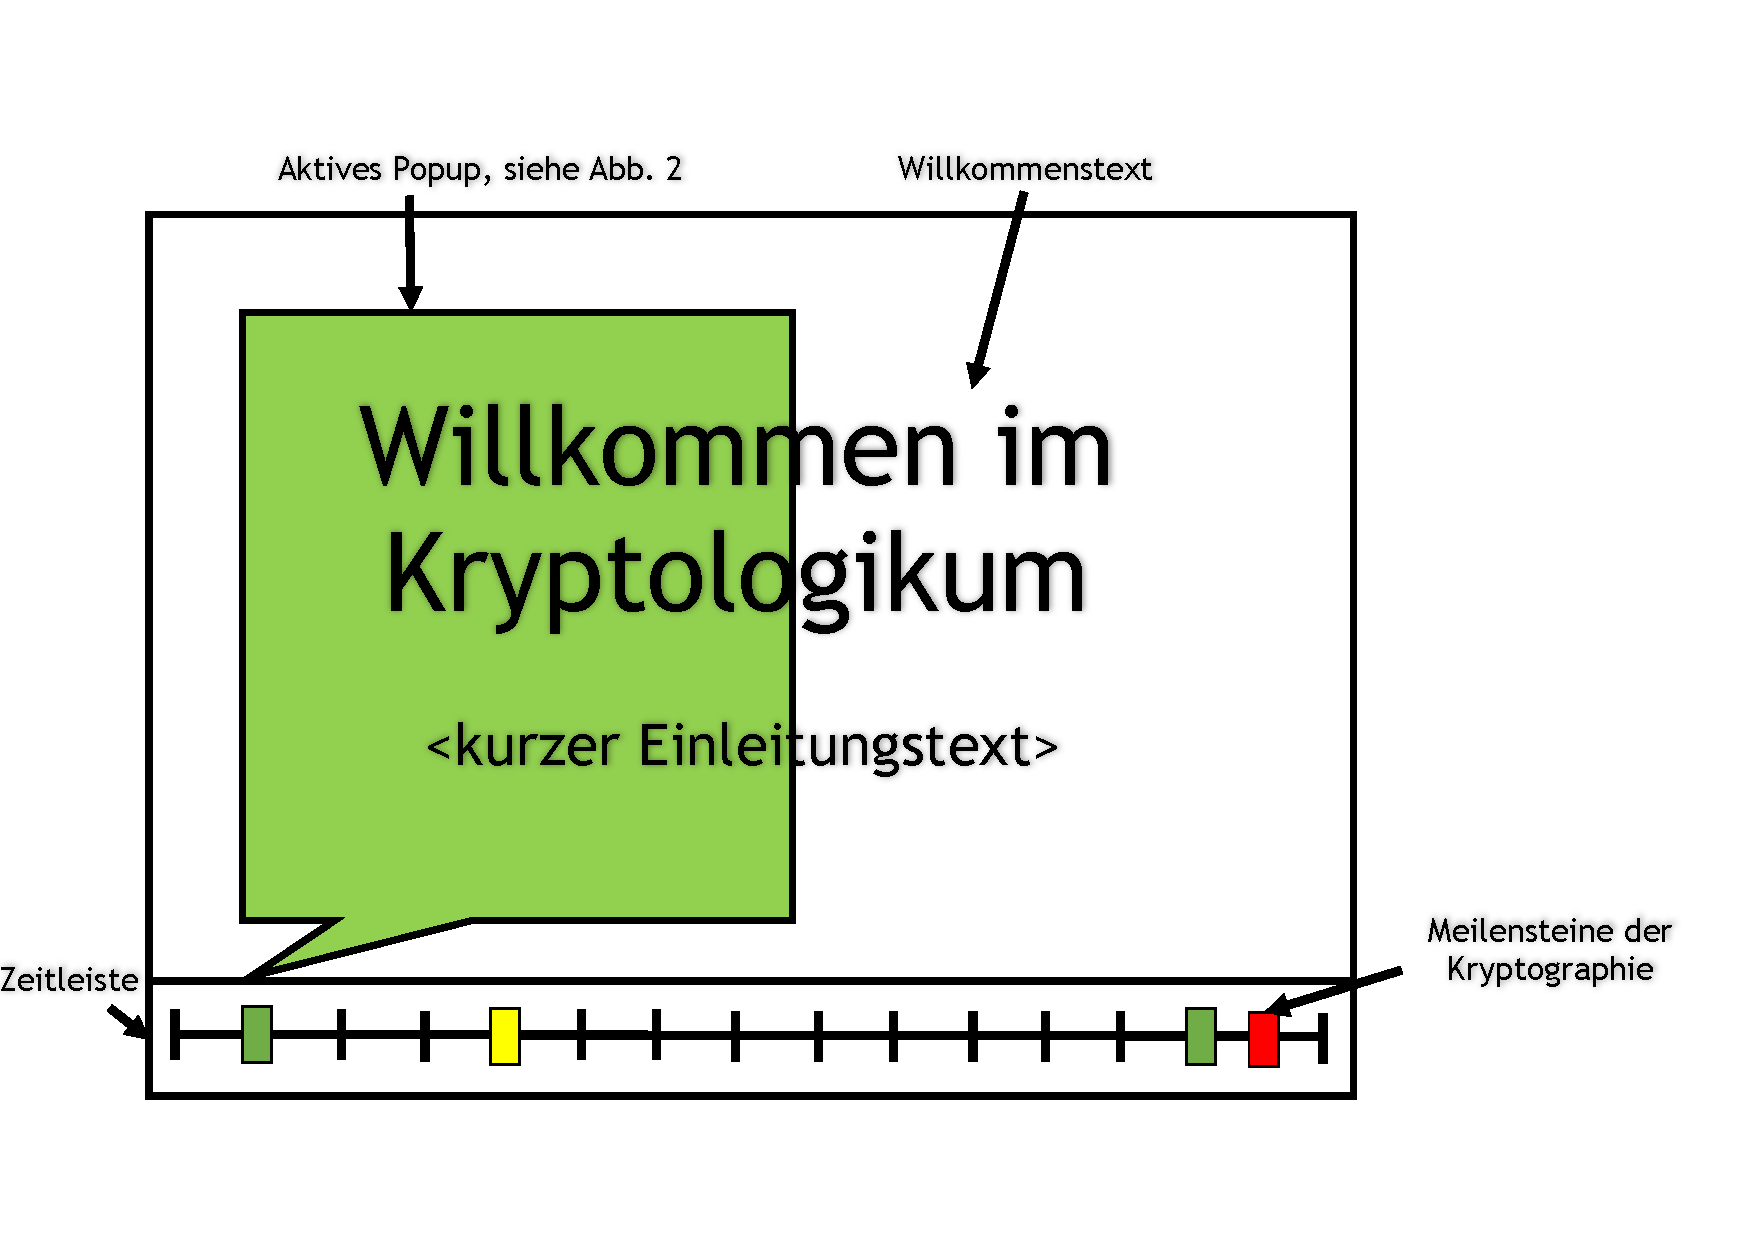
\includegraphics[width=\textwidth]{resources/ui_walkthrough_start-draft}
  \caption{Startbildschirm mit Zeitleiste.}
\end{figure}

Sobald ein Meilenstein ausgewählt wurde, erscheint ein Popover (Abb. 2), das den Namen, die Schwierigkeit und den Zweck des gewählten kryptografischen Verfahrens noch einmal zusammenfasst. Weiterhin wird ein Button dargestellt, welcher die Visualisierung startet.

\begin{figure}[H]
  \centering
    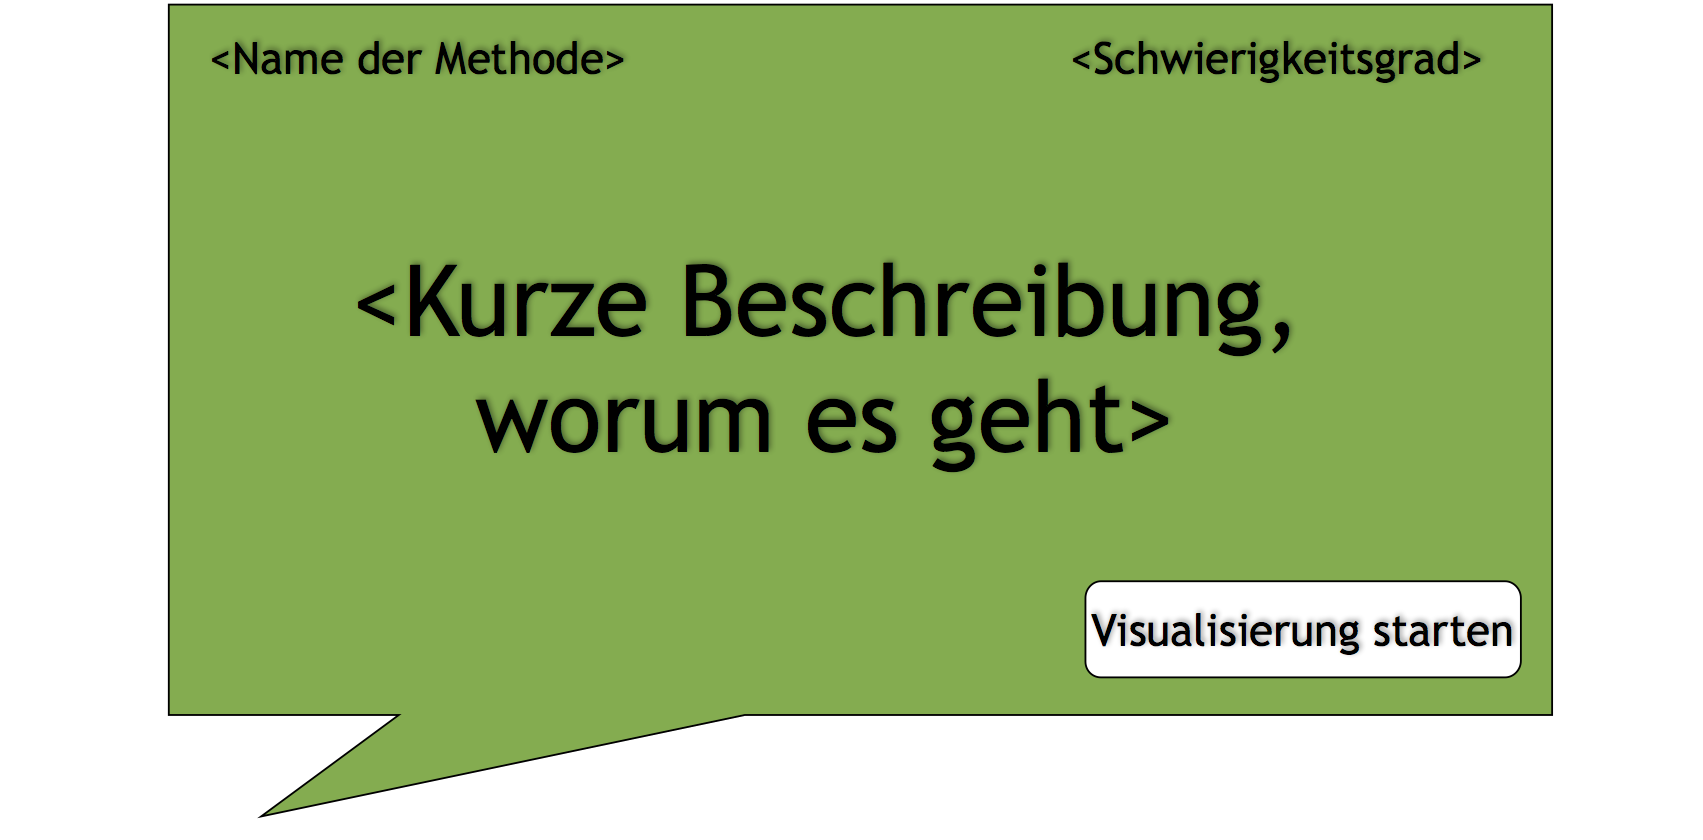
\includegraphics[width=\textwidth]{resources/ui_walkthrough_popover-draft}
  \caption{Detailansicht des Popovers in Abb 1.}
\end{figure}

Nachdem der Benutzer eine Visualisierung gestartet hat, wird diese angezeigt (Abb. 3). Hierbei ist hervorzuheben, dass der Benutzer zu jedem Zeitpunkt die Visualisierung abbrechen kann, indem er auf den Button in der oberen linken Ecke klickt. Hilfe erhält er zu jedem Zeitpunkt im rechten oberen Eck.

\begin{figure}[H]
  \centering
    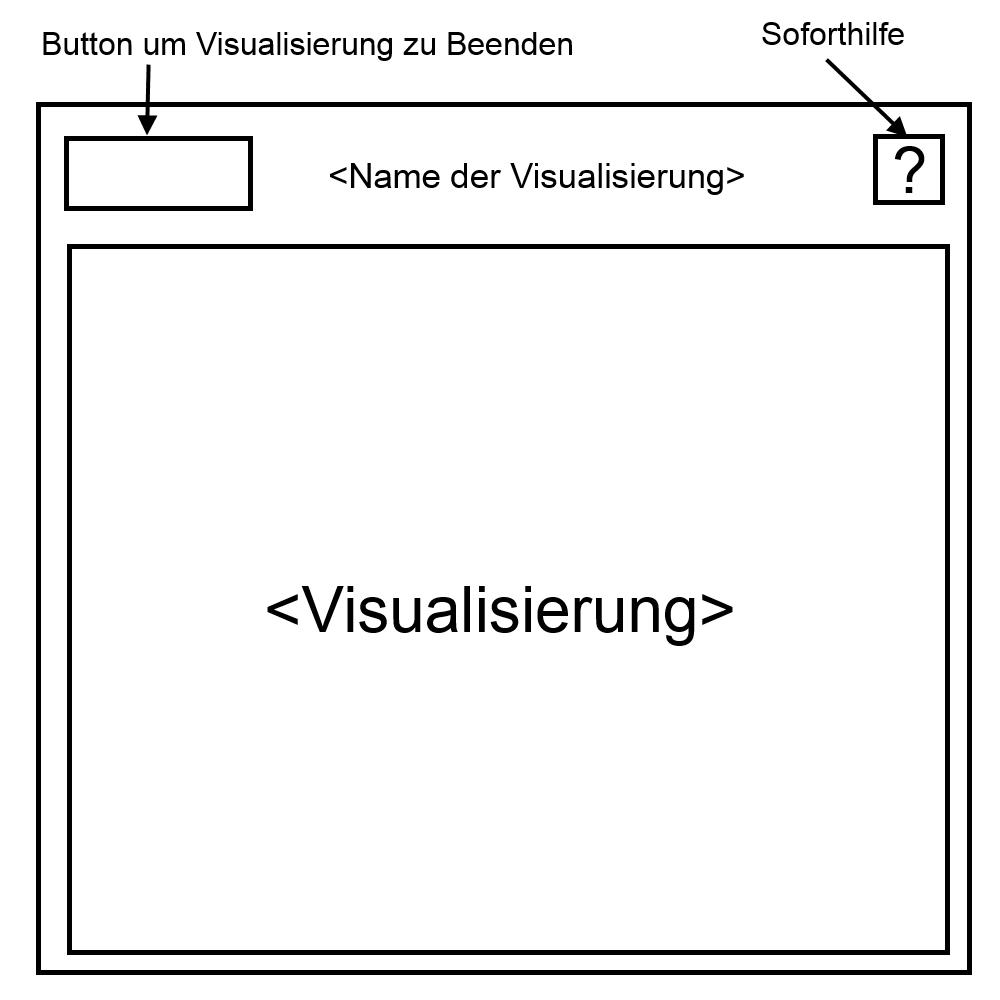
\includegraphics[width=\textwidth]{resources/ui_walkthrough_visualisation-draft}
  \caption{Darstellung einer Visualisierung.}
\end{figure}

Falls der Benutzer die Visualisierung erfolgreich beendet hat, wird Abb. 4 angezeigt. Zunächst wird dem Benutzer zu seinem Erfolg gratuliert. Weiterhin besteht die gut sichtbare Möglichkeit, zum Startbildschirm zurückzukehren. Falls das Interesse des Benutzers geweckt wurde, kann er zu den weiterführenden Informationen wechseln (Abb. 5).

\begin{figure}[H]
  \centering
    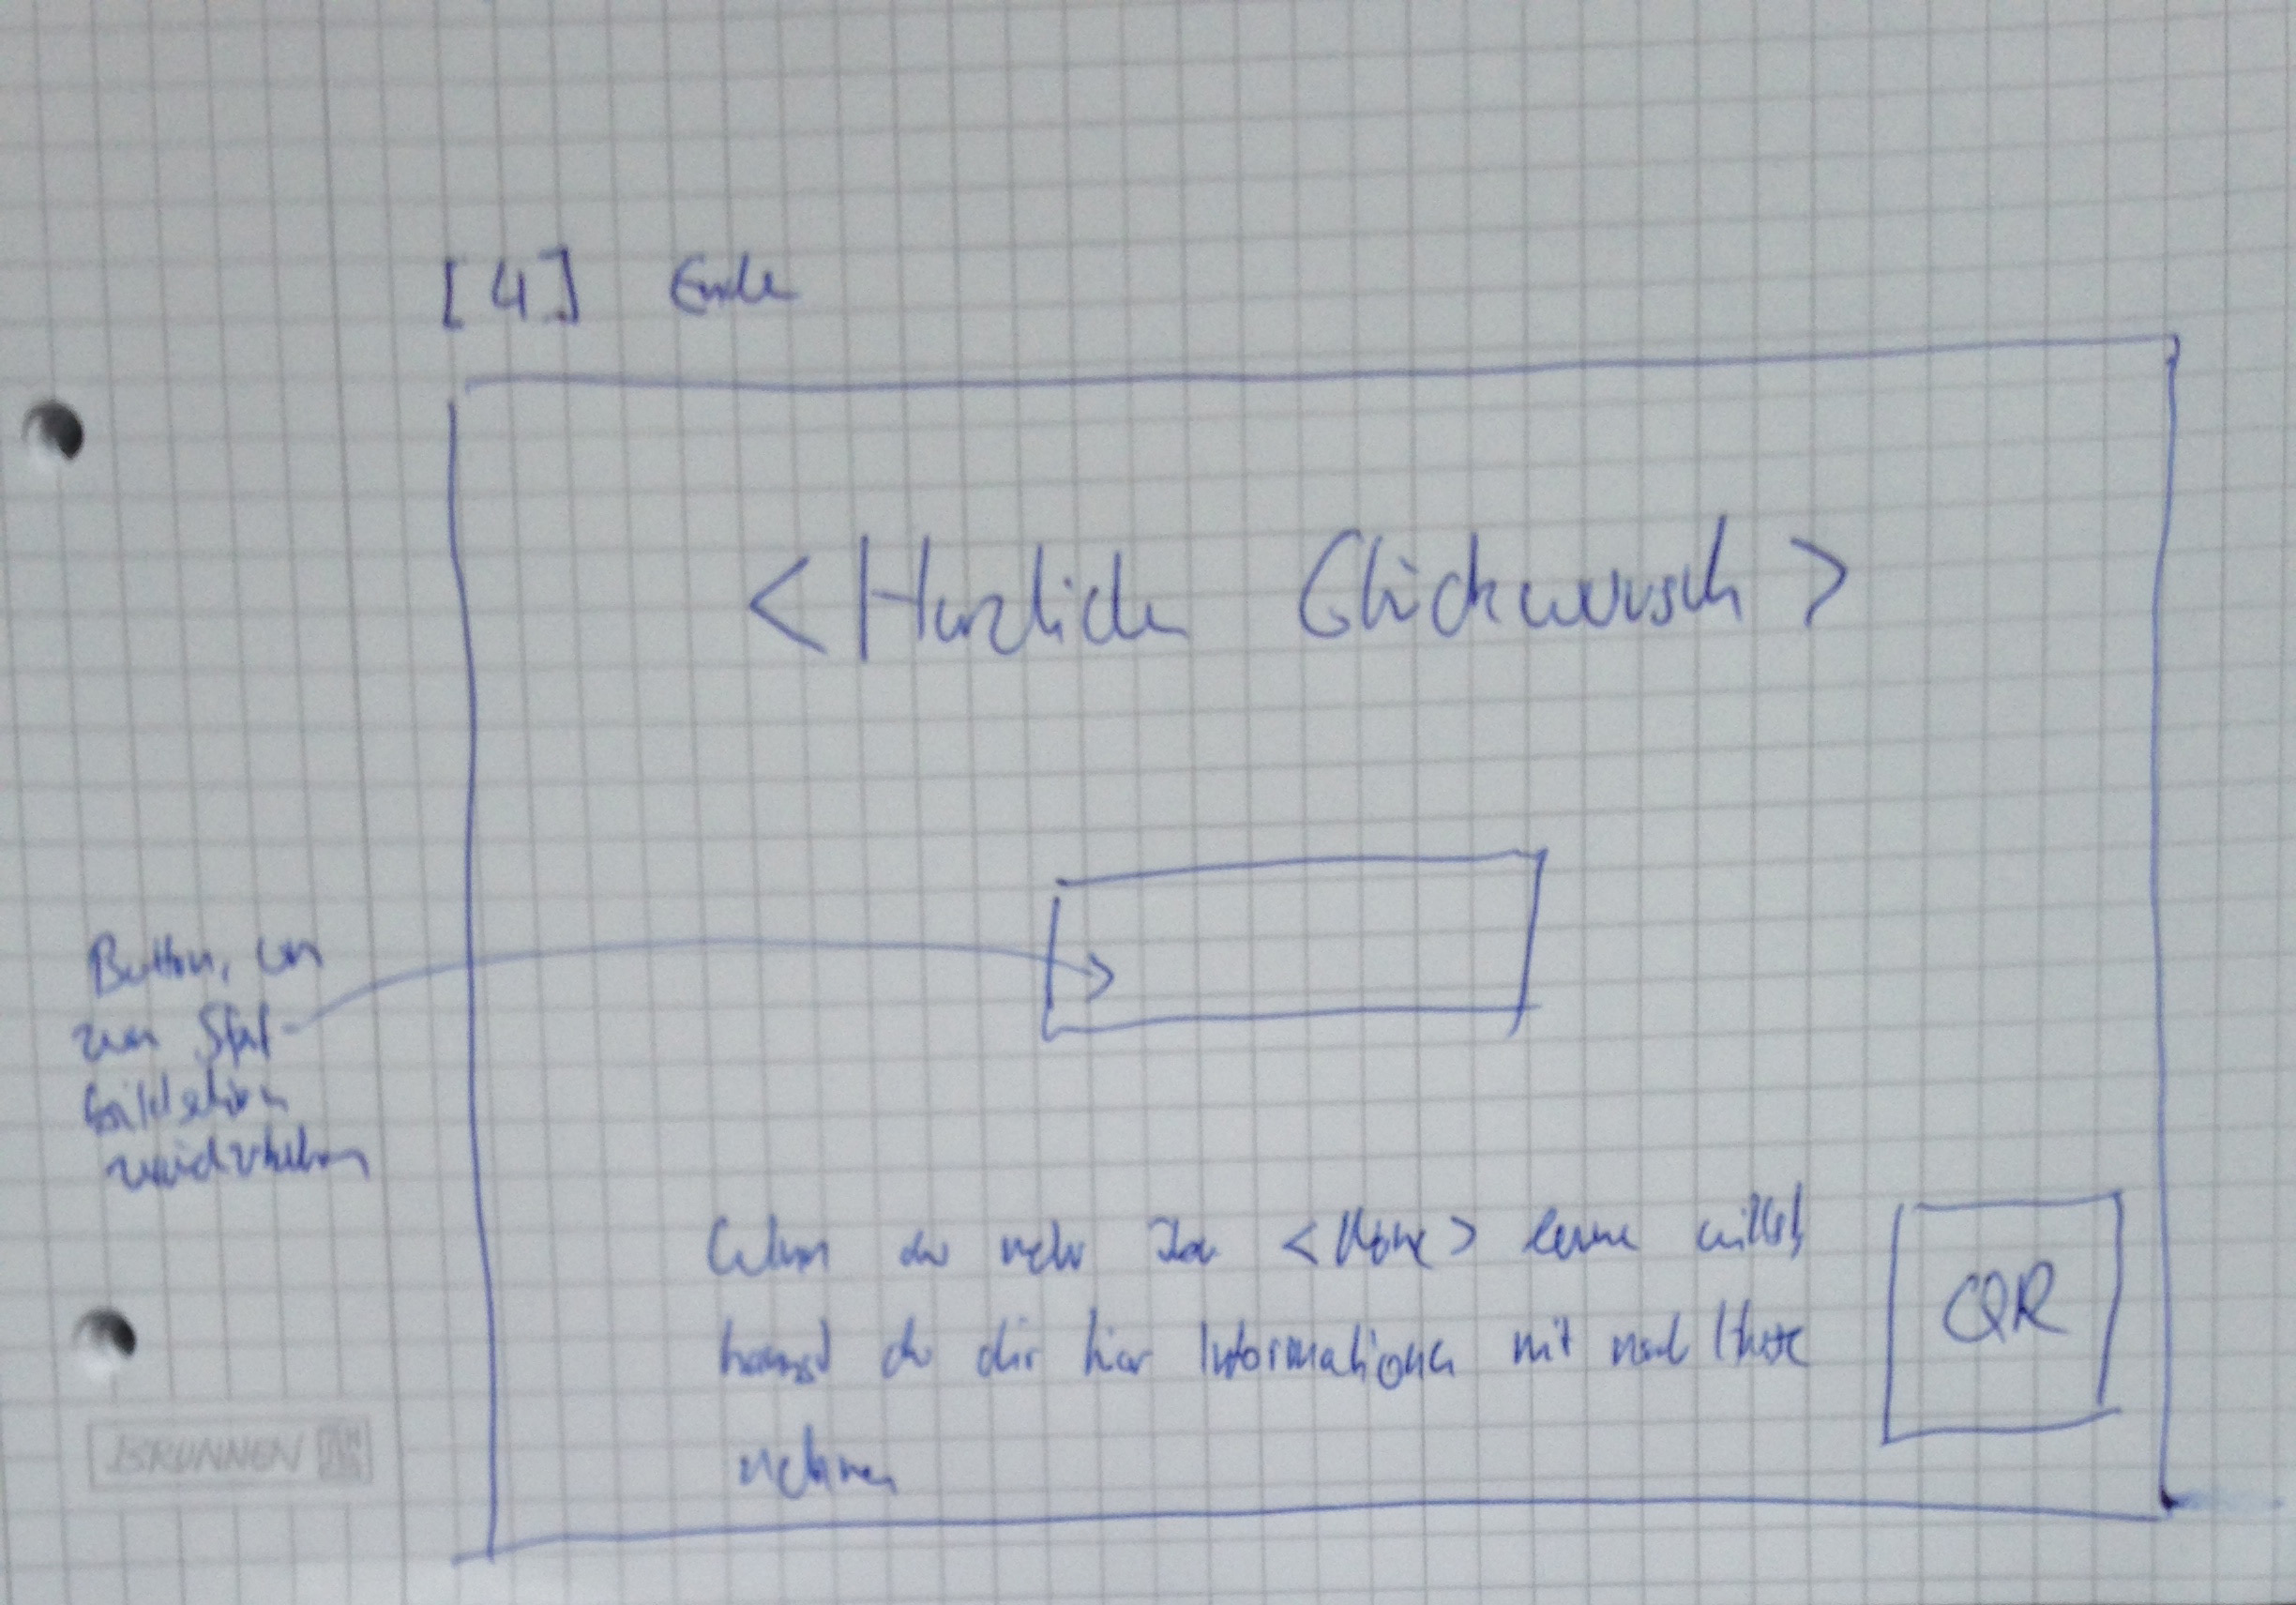
\includegraphics[width=\textwidth]{resources/ui_walkthrough_end-draft}
  \caption{Erfolgreiches Beenden einer Visualisierung.}
\end{figure}

Neben den weiterführenden Informationen wird auch ein QR-Code angezeigt. Dieser kann vom Benutzer gescannt werden, um weiterführende Links oder Literaturhinweise mit nachhause zu nehmen. Auch hier existiert die Möglichkeit, zum Startbildschirm zurückzukehren.

\begin{figure}[H]
  \centering
    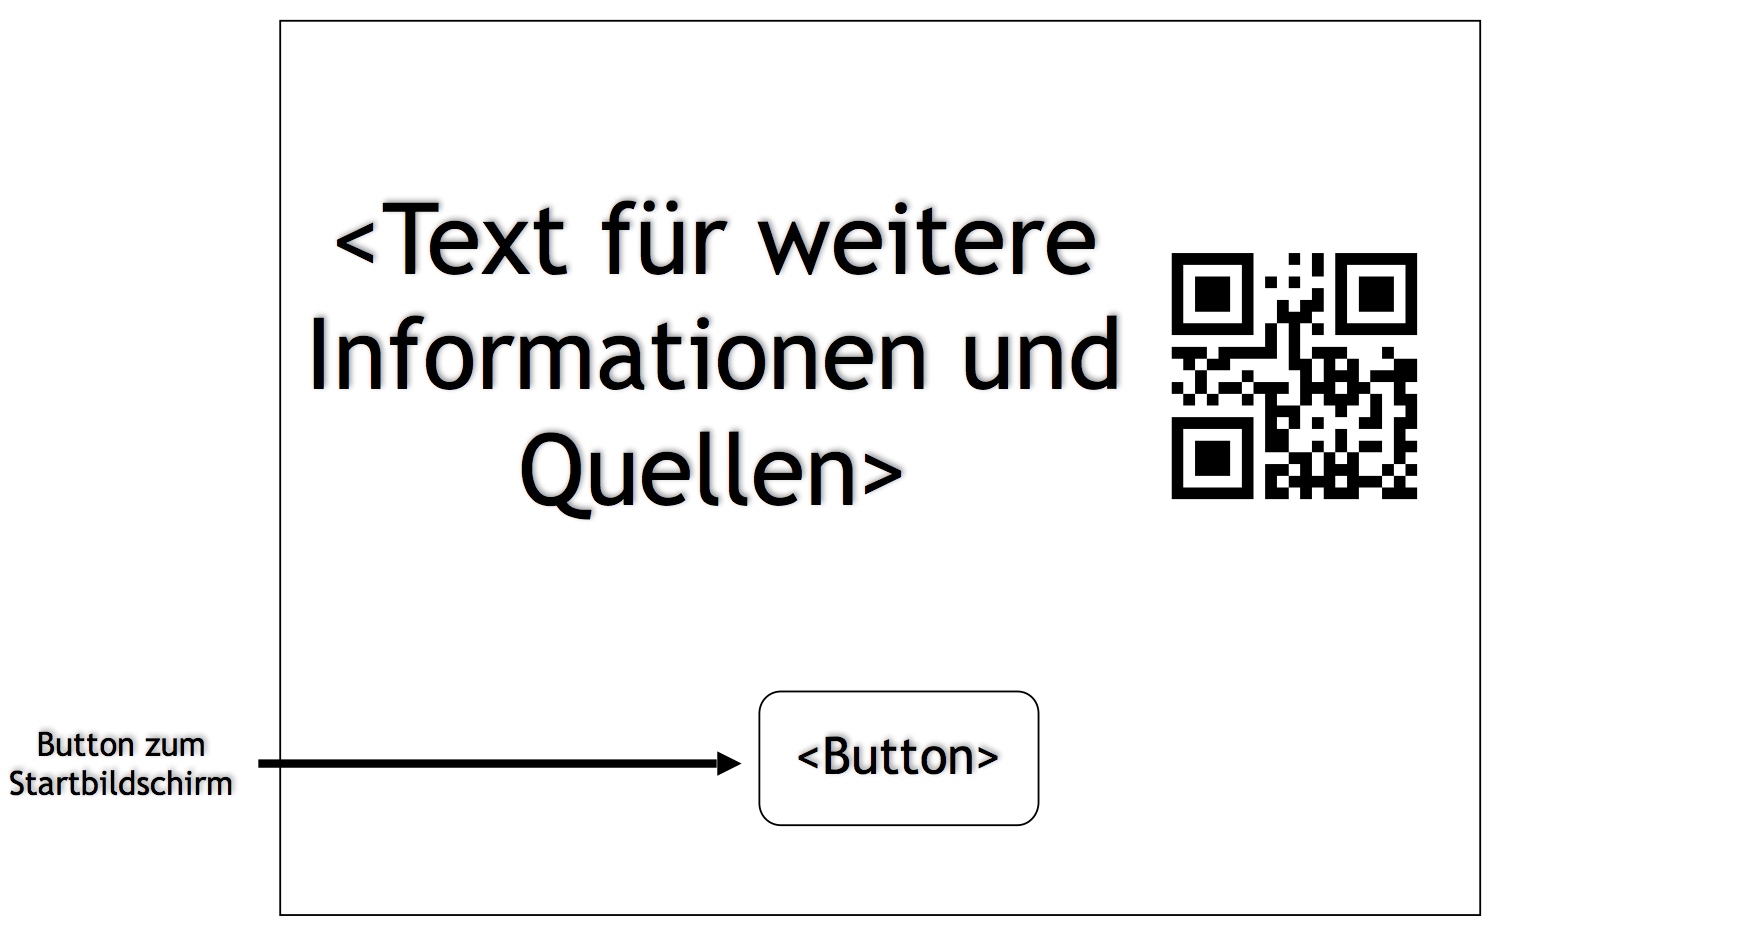
\includegraphics[width=\textwidth]{resources/ui_walkthrough_other}
  \caption{Weiterführende Informationen.}
\end{figure}


\section{Systemmodelle}

\subsection{Systemübersicht}
Das System verwendet das bekannte \gls{MVC}-Entwurfsmuster. Weiterhin ist geplant, das System in zwei Schichten zu unterteilen. Von unten nach oben enthält Schicht 1 wiederverwendbare und in sich abgeschlossene Bibliotheken. Zum einen handelt es sich hierbei um Code von Dritten (z.B. um QR-Codes zu generieren). Weiterhin ist eine Sammlung wiederverwendbarer Klassen (nachfolgend \gls{GraphicsLib} genannt) geplant. \gls{GraphicsLib} wird vor allem aus \gls{UI}-Elementen bestehen, die für die Implementierung aller Visualisierungen wertvoll sind.

\begin{figure}[H]
  \centering
    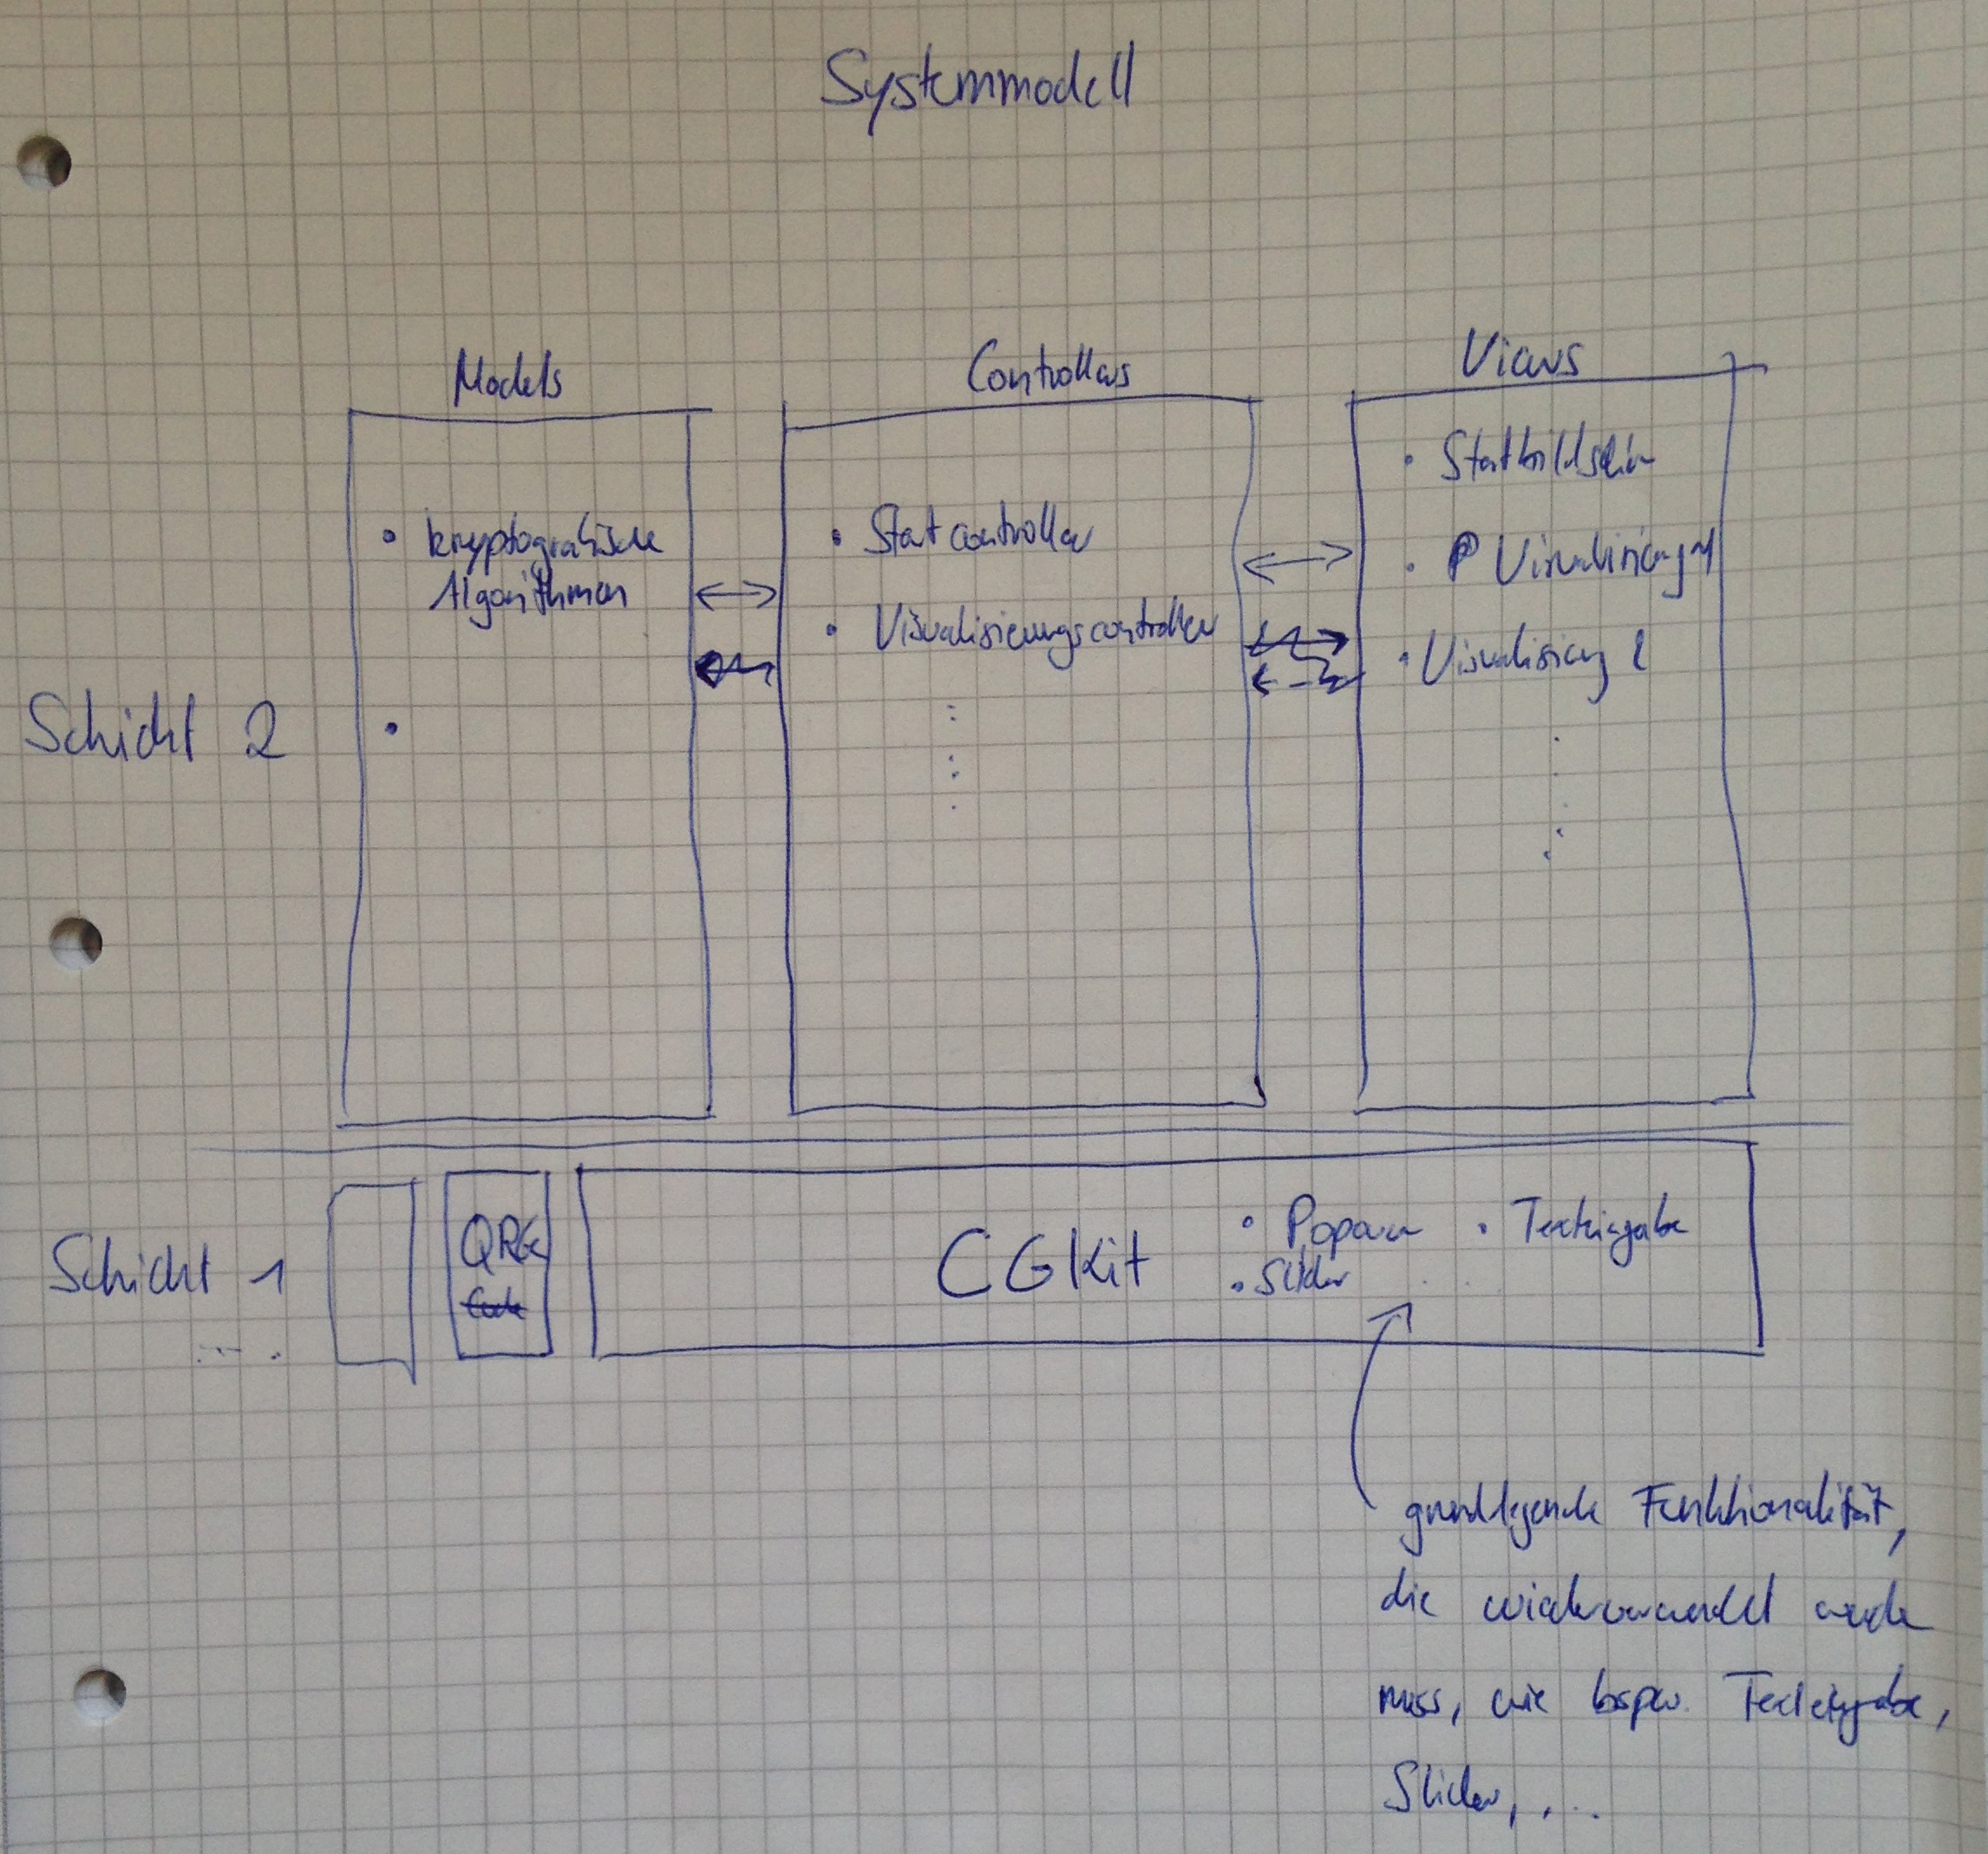
\includegraphics[width=\textwidth]{resources/systemmodel-draft}
  \caption{Schematische Darstellung des beschriebenen Systems.}
\end{figure}


\section{Testszenarien}

\textbf{Szenario 1}:
Bob ist interessiert an Kryptographie und besucht aus diesem Grund das \gls{Kryptologikum}. Er nähert sich dem \gls{Cryptographics}-Ausstellungsstück. Eine Berührung des Bildschirmes zeigt den Startbildschirm von \gls{Cryptographics}: Eine Zeitleiste, auf dem chronologisch angeordnet verschiedene kryptographische Verfahren dargestellt werden. Die Verfahren sind außerdem farblich durch ihre Komplexität von grün (leicht) bis rot (schwer) gekennzeichnet. Bob wählt durch eine Berührung die Caesar-Chiffre aus, sie befindet sich nämlich am Anfang der Zeitleiste. Daraufhin erscheint eine kurze Einleitung. Nach dem Durchlesen der Einleitung starten Bob die Visualisierung. Die folgende Demonstration der Caesar-Chiffre erfolgt Schritt für 
Schritt auf 
einer speziell für das Verfahren ausgelegten Oberfläche. Auf genau dieser Oberfläche kann Bob nach dem Beispiel sein neu erlerntes Wissen über das Verfahren anwenden, um Texte zu verschlüsseln, und durch einen gegebenen Schlüssel zu entschlüsseln. Nachdem Bob das Verfahren verstanden hat, kehrt Bob zum Startbildschirm zurück. Da er auch an den anderen Verfahren interessiert ist, arbeitet er sich am Zeitstrahl entlang durch das Programm. Schließlich stößt er auf das Diffie-Hellman-Verfahren, über welches er zusätzliche Informationen erhalten möchte. Er berührt einen dafür vorgesehenen Button und landet auf einem Bildschirm, der weiterführende Informationen sowie einen QR-Code anzeigt. Bob liest die weiterführenden Informationen und scant den QR-Code mit seinem Smartphone. Auch zuhause kann sich Bob dank des gescannten QR-Codes weiter über das Diffie-Hellman-Verfahren informieren.\\

\textbf{Szenario 2}:
Die ungeduldige Alice wurde von ihrer Freundin überredet an der Ausstellung teilzunehmen. Sie sieht das \gls{Cryptographics}-Ausstellungsstück und versucht es durch wiederholte zufällige Eingaben zum Absturz zu bringen. Das Programm erweist sich jedoch schnell als zu robust. Schließlich wählt sie das komplizierteste kryptographische Verfahren aus, um nachfolgenden Besuchern den Einstieg zu erschweren. Nachdem sie gegangen ist, muss sie jedoch enttäuscht feststellen, dass der nächste Besucher keine weitere Schwierigkeiten hat, das Programm mit dem dafür vorgesehenen Button in den Grundzustand zurückzuversetzen.\\

\textbf{Szenario 3}:
Nachdem Bob nun längere Zeit am \gls{Cryptographics}-Ausstellungs\-stück verbracht hat, blickt er erschrocken auf die Uhr und stellt fest, dass es schon viel zu spät geworden ist. Er bricht auf und lässt das Programm genau so zurück, wie er es gerade eben noch benutzt hat. Nach seiner letzten Interaktion erscheint nach x Sekunden eine Meldung, die Bob darauf hingewiesen hätte, dass sich das Programm bald zurücksetzt, sollte in den nächsten y Sekunden keine Eingabe mehr erfolgen. Da er jedoch schon an der Bushaltestelle steht, wechselt \gls{Cryptographics} automatisch zurück zum Startbildschirm.\\

\textbf{Szenario 4}:
Die Ausstellung ist für diesen Tag zu Ende, und die Krypto\-lo\-gi\-kum-Administratorin Claudia schließt gerade noch die Tür hinter Bob ab, um sich jetzt den strombetriebenen Exponaten zu widmen. Als sie am \gls{Cryptographics}-Ausstellungsstück ankommt, versucht sie zunächst, irgendwie zum Betriebssystem zurückzukehren, um den PC sicher herunterfahren zu können. Nach kurzer Zeit stellt sie fest, dass das ohne eine eingesteckte Hardware-Tastatur auf keinen Fall möglich ist. Sie holt also eine USB-Tastatur, steckt sie ein, kehrt über den Windows-Taskmanager zum Betriebssystem zurück, fährt den PC herunter und macht die Lichter aus.\\

\begin{figure}[H]
  \centering
    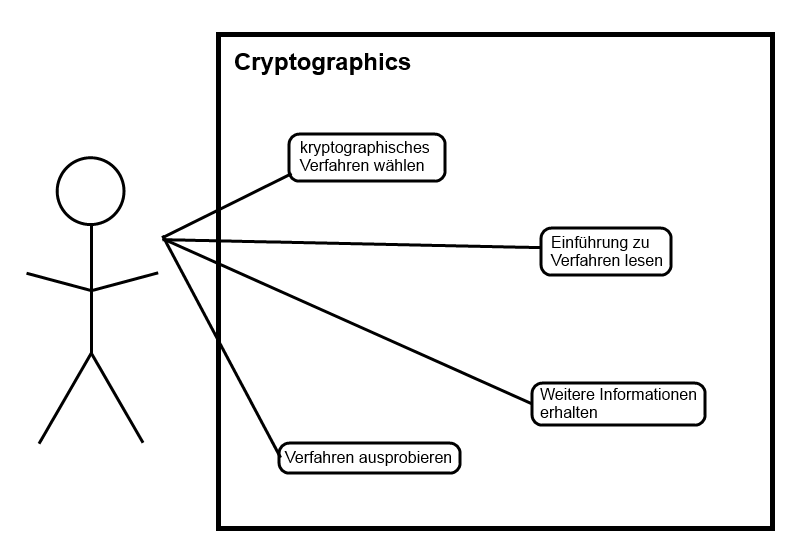
\includegraphics[width=\textwidth]{resources/usecase1}
  \caption{Anwendungsfalldiagramm zu beschriebenen Szenarien.}
\end{figure}

\section{Globale Testfälle}
\begin{T}[start = 10]
\item Beim Drücken des Hilfe-Buttons bekommt der Nutzer Hilfestellungen zur aktuellen Aufgabe.
\end{T}

\begin{T}[start = 20]
 \item Benutzer muss eine Farbe für Alice beim Diffie-Hellman-Schlüsselaustausch auswählen. Diese wird dann visuell im Bildschirm zugehörig zu Alice als ``öffentliche'' Farbe abgebildet.
\end{T}

\begin{T}[start = 30]
 \item Nach dem Auswählen der geheimen Farbe beim Diffie-Hellman-Schlüssel\-aus\-tausch für Alice, wird dieser visuell mit der zuvor gewählten, öffentlichen Farbe gemischt und am Bildschirm dargestellt.
\end{T}

\begin{T}[start = 40]
 \item Je nachdem welche Farbe (öffentlich, nicht-öffentlich oder gemischt) der Nutzer zum Schicken an Bob beim Diffie-Hellman-Schlüsselaustausch auswählt, wird der Nutzer darüber informiert ob seine Aktion falsch oder richtig war.
\end{T}

\begin{T}[start = 50]
 \item Bei Caesar und Vigenère kann der Benutzer über ein Eingabefenster Eingaben tätigen.
\end{T}

\begin{T}[start = 60]
 \item Bei Caesar und Vigenère kann der Benutzer sich die Eingaben generieren lassen.
\end{T}

\begin{T}[start = 70]
 \item Im Laufe des Selbstversuchs von Vigenère und Caesar sollen die Buchstaben der Aufgabe aufleuchten.
\end{T}

\begin{T}[start = 80]
 \item Im Laufe des Selbstversuchs von Vigenère und Caesar soll das Alphabet interaktiv sein.
\end{T}

\begin{T}[start = 90]
 \item Die Anwendung muss am Ende vom Schritt 1 der Phase 2, Selbstversuch bei Caesar und Vigenère den vom 
       Benutzer verschlüsselten Klartext entschlüsseln und das Ergebnis anzeigen.
\end{T}

\begin{T}[start = 100]
 \item Am Ende des 2ten Schritt der Phase 2, Selbstversuch soll bei Caesar und Vigenère die Anwendung den entschlüsselten Klartext 
       auf Richtigkeit prüfen und es dem Benutzer anzeigen.
\end{T}

\begin{T}[start = 110]
 \item Im 3ten Schritt der Phase 2, Selbstversuch soll der Benutzer sich nach der Demonstration Histogramme erstellen lassen können.
\end{T}

\begin{T}[start = 120]
 \item Am Ende jeder Phase soll bei Caesar und Vigenère die Anwendung automatisch in die nächste Phase übergehen und sich die Oberfläche 
       der nächsten Phase entsprechend ändern.
\end{T}

\section{Qualitätsbestimmung}

Die hier aufgeführten Merkmale richten sich nach dem ISO/IEC 9126-Standard\footnote{\url{http://de.wikipedia.org/wiki/ISO/IEC_9126}}.

% As specified by http://de.wikipedia.org/wiki/ISO/IEC_9126
\begin{table}[H]
  \begin{tabular}{| l | c | c | c | c |}
    \hline
     & \textbf{sehr wichtig} & \textbf{wichtig} & \textbf{neutral} & \textbf{unwichtig} \\ \hline
    \textbf{Funktionalität} &  &  &  & \\ \hline
    \gls{Angemessenheit} &  &  & \xmark & \\ \hline
    \gls{Richtigkeit} &  & \xmark &  & \\ \hline
    \gls{Interoperabilitaet} &  &  &  & \xmark \\ \hline
    \gls{Ordnungsmaessigkeit} &  &  & \xmark & \\ \hline
    \gls{Sicherheit} &  &  & \xmark & \\ \hline
     &  &  &  & \\ \hline
    \textbf{Zuverlässigkeit} &  &  &  & \\ \hline
    \gls{Reife} & & \xmark &  & \\ \hline
    \gls{Fehlertoleranz} & & \xmark &  & \\ \hline
    \gls{Wiederherstellbarkeit} &  &  & \xmark & \\ \hline
     &  &  &  & \\ \hline
    \textbf{Benutzbarkeit} &  &  &  & \\ \hline
    \gls{Verstaendlichkeit} & \xmark &  &  & \\ \hline
    \gls{Erlernbarkeit} & \xmark &  &  & \\ \hline
    \gls{Bedienbarkeit} & \xmark &  &  & \\ \hline
     &  &  &  & \\ \hline
    \textbf{Effizienz} &  &  &  & \\ \hline
    \gls{Zeitverhalten} &  &  & \xmark & \\ \hline
    \gls{Verbrauchsverhalten} &  &  & \xmark & \\ \hline
     &  &  &  & \\ \hline
    \textbf{Änderbarkeit} &  &  & \xmark & \\ \hline
    \gls{Analysierbarkeit} &  &  &  & \\ \hline
    \gls{Modifizierbarkeit} &  & \xmark &  & \\ \hline
    \gls{Stabilitaet} &  &  & \xmark & \\ \hline
    \gls{Pruefbarkeit} &  &  & \xmark & \\ \hline
     &  &  &  & \\ \hline
    \textbf{Übertragbarkeit} &  &  &  & \\ \hline
    \gls{Anpassbarkeit} &  &  & \xmark & \\ \hline
    \gls{Installierbarkeit} &  &  & \xmark & \\ \hline
    \gls{Konformitaet} &  &  & \xmark & \\ \hline
    \gls{Austauschbarkeit} &  &  & \xmark & \\ \hline
    \end{tabular}
\end{table}

Zusammenfassend lässt sich sagen, dass vor allem die Benutzbarkeit eintscheidend ist.


\section{Anhang}

%Glossar ausgeben
\glsaddall
\printglossary[numberedsection, style=altlist]

\end{document}
